 
\documentclass{beamer}

\usepackage{tikz}
\usetikzlibrary{arrows}

\usepackage{amsmath}

\title{Brain mapping tools for neuroscience research}
\author{Daniel Tward (\texttt{dtward@cis.jhu.edu})}
\date{}

\institute{NeuroData and Center for Imaging Science\\
Department of Biomedical Engineering\\
Johns Hopkins University}


\usetheme{default}
%\renewcommand{\insertnavigation}[1]{}
\setbeamertemplate{headline}{}
\setbeamertemplate{footline}[text line]{%
  \parbox{\linewidth}{Daniel Tward (\texttt{dtward@cis.jhu.edu}) \hfill Johns Hopkins University \hfill Brain mapping tools for neuroscience research}}
  
\beamertemplatenavigationsymbolsempty
\renewcommand{\footnotesize}{\tiny}

\begin{document}
\begin{frame}
\maketitle
\end{frame}



%\begin{frame}{What is brain mapping?}
%
%Assigning a standard coordinate to each point in a neuroimage.
%
%I think this is a very weak first slide
%
%\end{frame}


\begin{frame}{The goal of brain mapping}

%Registration: , Annotation: , Morphometry: 


% my picture will have an target (top left), a atlas (top right), and a deformation (bottom center)

\begin{tikzpicture}
\tikzstyle{rect} = [rectangle, thick, minimum width=2cm, minimum height=2cm, text centered, text width=3.5cm, draw=black, fill=black!10];
\tikzstyle{arrow} = [->, thick, line width=1mm];

\node (target) [rect ] at (-3.5,0) {Experimental data 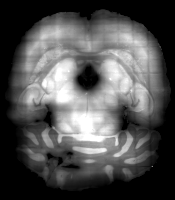
\includegraphics[width=\textwidth]{ex1_target_slice.png}};
\node (atlas) [rect]  at (3.5,0) {Standard coordinates 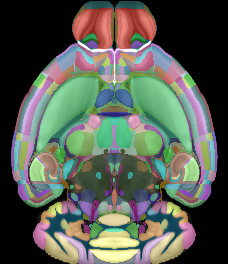
\includegraphics[width=\textwidth]{ex1_allen_slice.png}};
\node (map) [rectangle, text width=3cm, text centered, ] at (0,-0) {3. Transformation 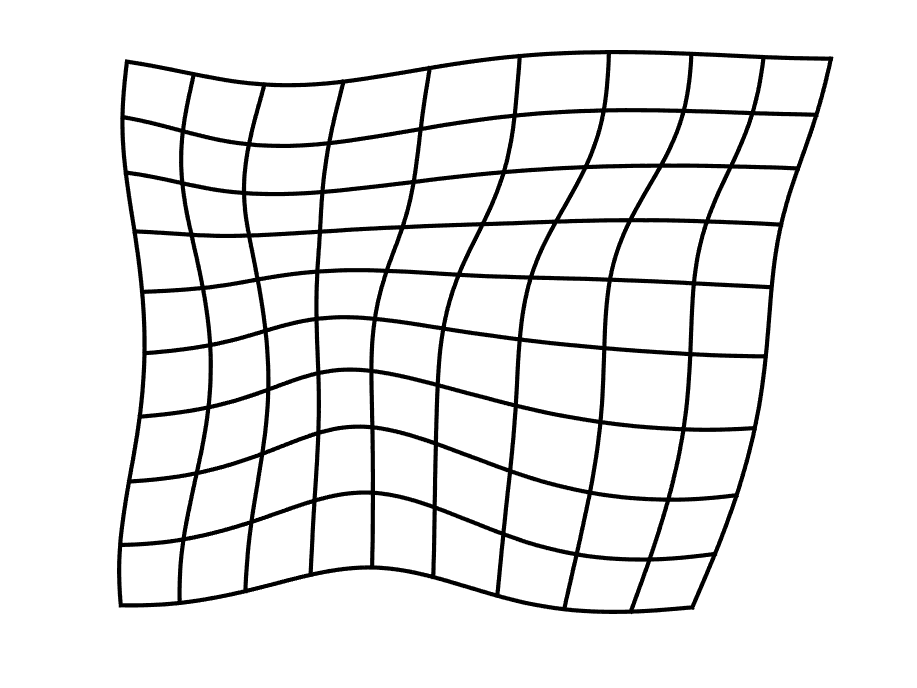
\includegraphics[width=2.75cm,clip,trim=0.5in 0in 0.5in 0in]{ex1_warp.png}};

\draw [arrow] (target) to [out=45,in=135] node [anchor=south] {1. Registration} (atlas);
\draw [arrow] (atlas) to [out=-135,in=-45] node [anchor=north] {2. Interpretation} (target);

\end{tikzpicture}
\end{frame}

\begin{frame}{1. Registration}



Align images into a standard coordinate system

\begin{tikzpicture}
\tikzstyle{rect} = [rectangle, thick, text centered, text width=1.4cm, fill=black!10];
\tikzstyle{arrow} = [->, thick, line width=0.5mm];


\node (mni) [rect] at (0,0) {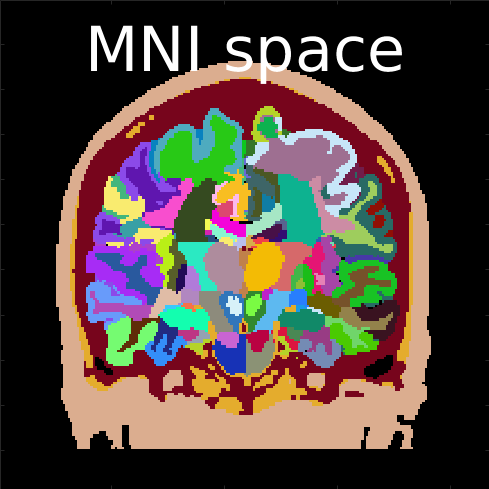
\includegraphics[width=\textwidth]{reg_mni}};



\node (im1a) [rect] at (-4.5,1) {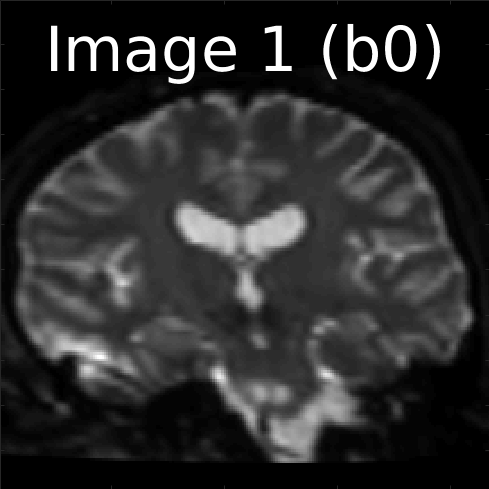
\includegraphics[width=\textwidth]{reg_1a}};



\node (im2a) [rect] at (4.5,1) {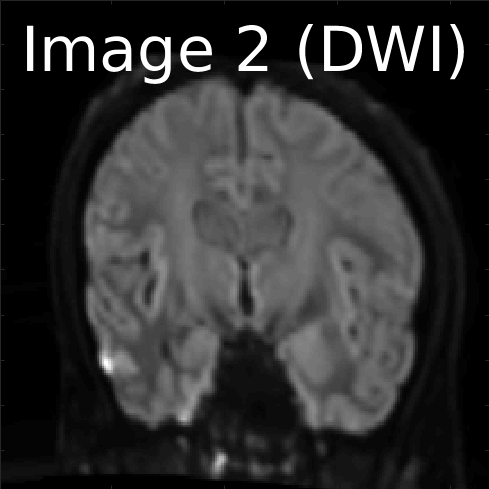
\includegraphics[width=\textwidth]{reg_2a}};



\node (im4a) [rect] at (4.5,-1) {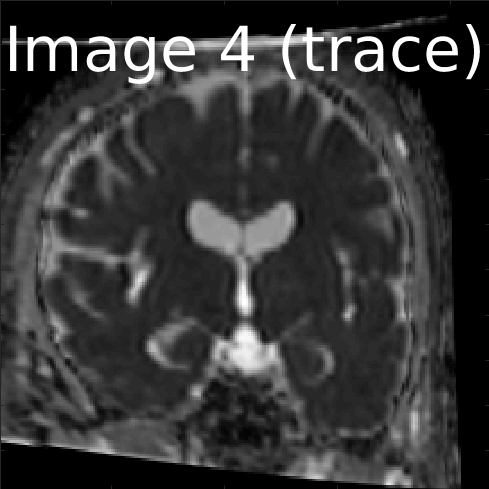
\includegraphics[width=\textwidth]{reg_4a}};


\node (im3a) [rect] at (-4.5,-1) {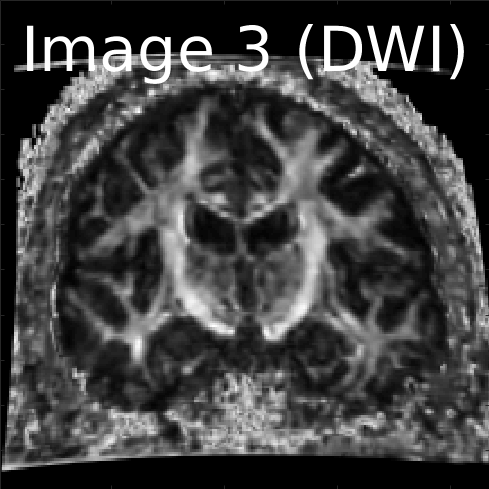
\includegraphics[width=\textwidth]{reg_3a}};

\draw [arrow](im1a) -- (mni);
\draw [arrow](im2a) -- (mni);
\draw [arrow](im3a) -- (mni);
\draw [arrow](im4a) -- (mni);


\uncover<2->{
\node (im2b) [rect] at (-2,0.9) {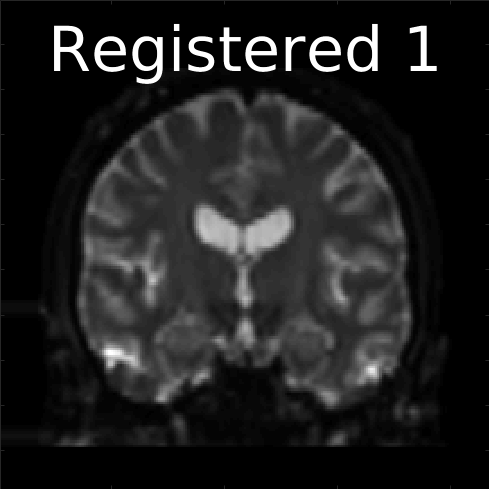
\includegraphics[width=\textwidth]{reg_1b}};
\node (im2b) [rect] at (2,0.9) {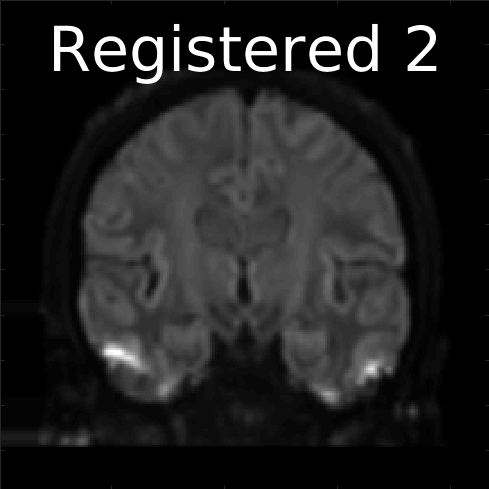
\includegraphics[width=\textwidth]{reg_2b}};
\node (im2b) [rect] at (2,-0.9) {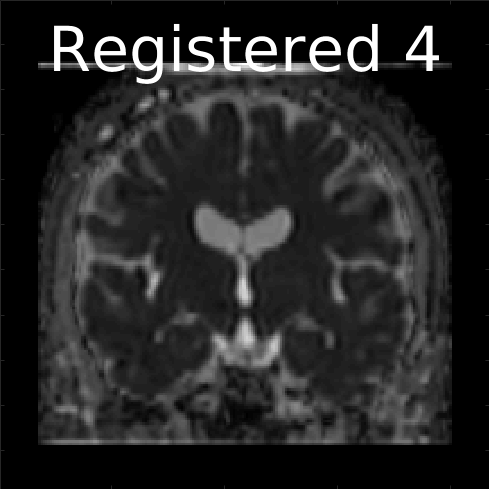
\includegraphics[width=\textwidth]{reg_4b}};
\node (im2b) [rect] at (-2,-0.9) {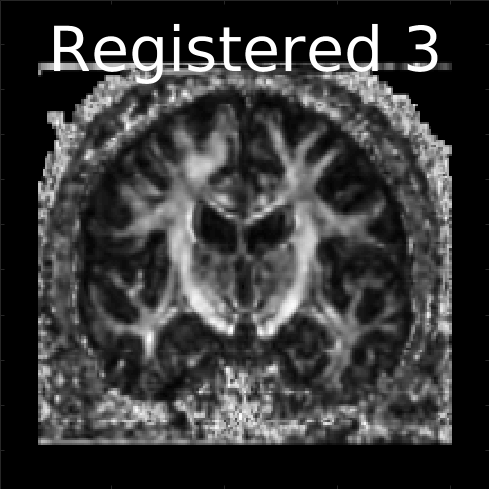
\includegraphics[width=\textwidth]{reg_3b}};
}
\end{tikzpicture}



\begin{itemize}
\item 
Enrich information by fusing modalities


\item
Analyze different specimens statistically

\item 
Build databases of information indexed to spatial coordinates

\end{itemize}

\end{frame}



\begin{frame}{2. Interpretation}


Leverage information stored in atlas coordinates.\footnote{MBA: Mouse brain architecture \url{brainarchitecture.org}, ARA: Allen reference atlas \url{connectivity.brain-map.org/}}

\begin{minipage}{0.3\textwidth}
MBA
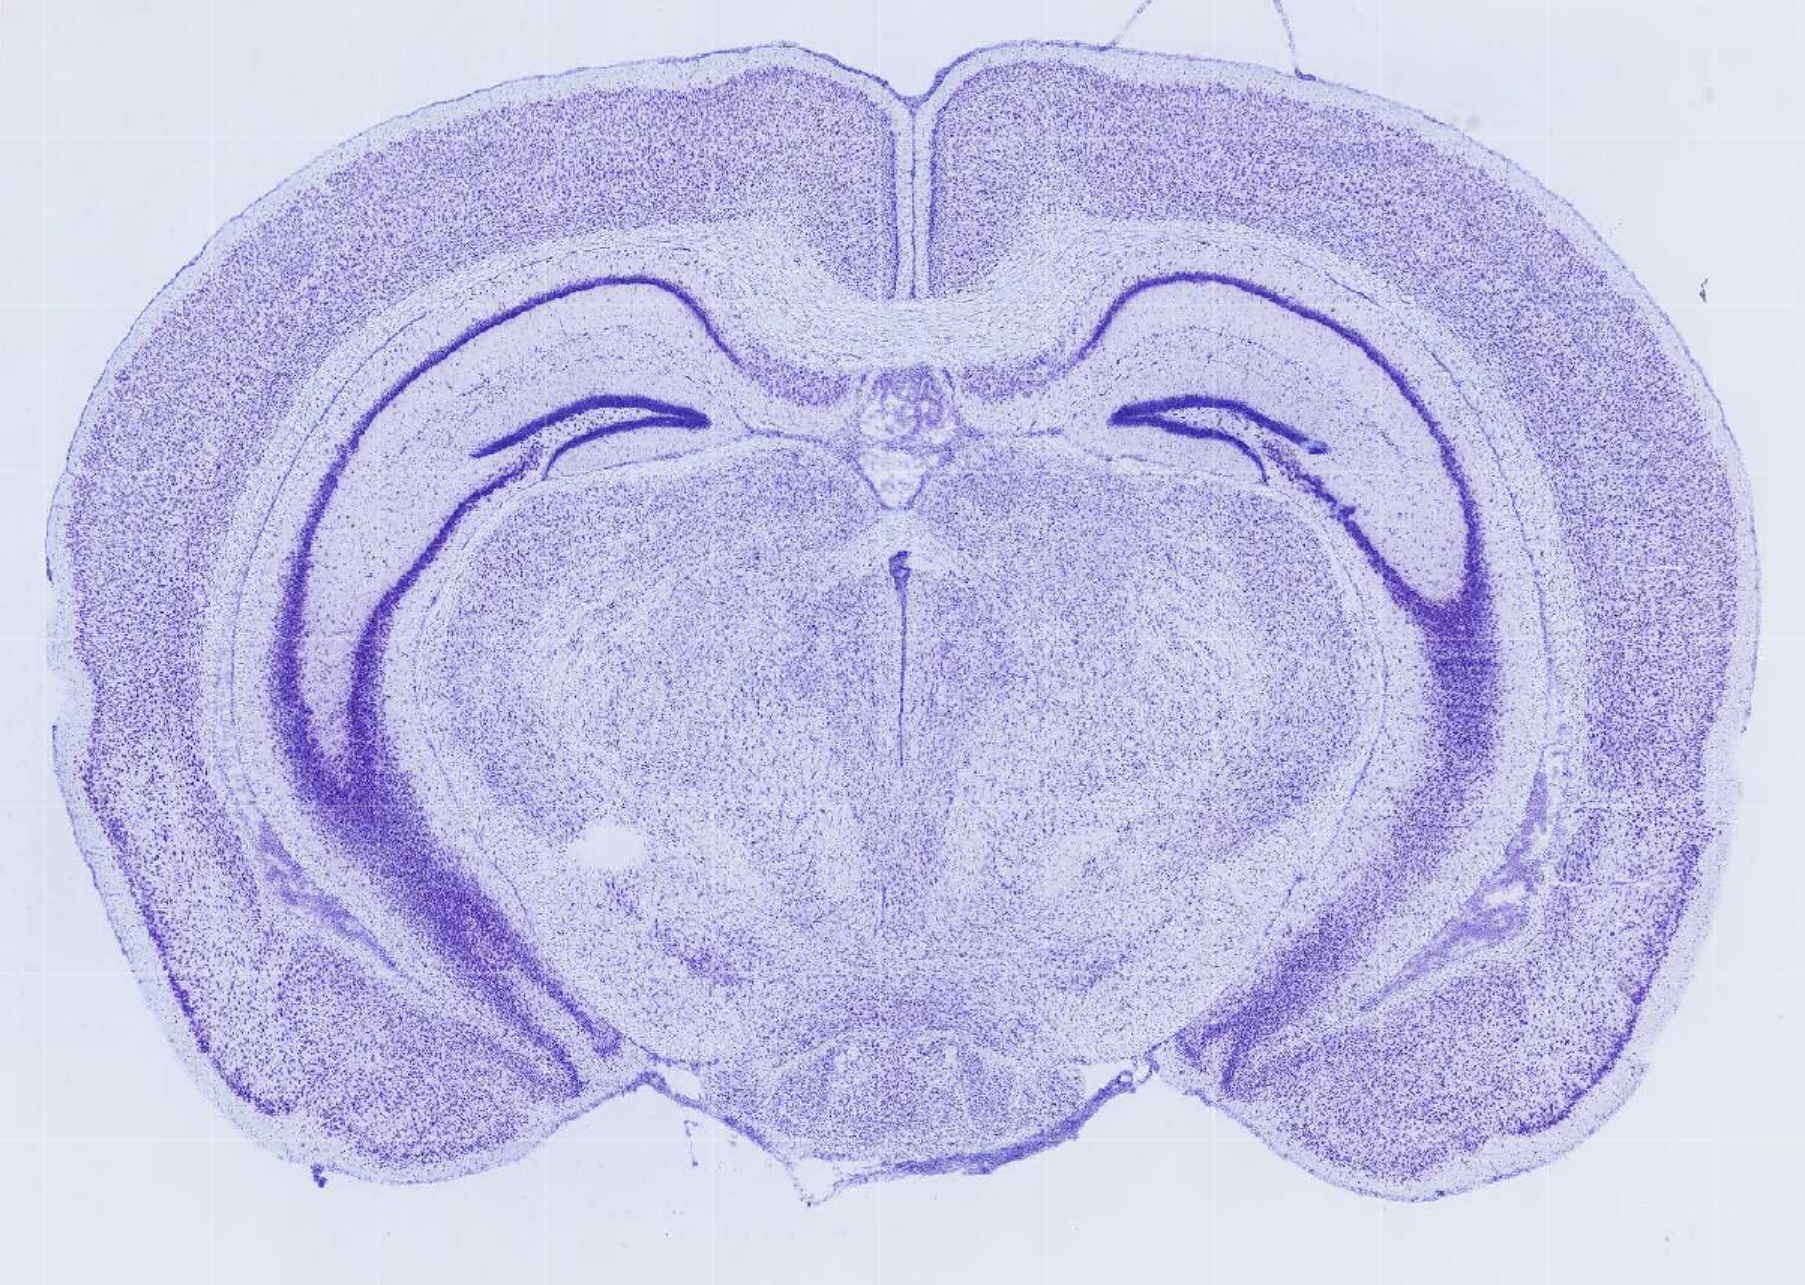
\includegraphics[width=\textwidth]{mba2.png}\\
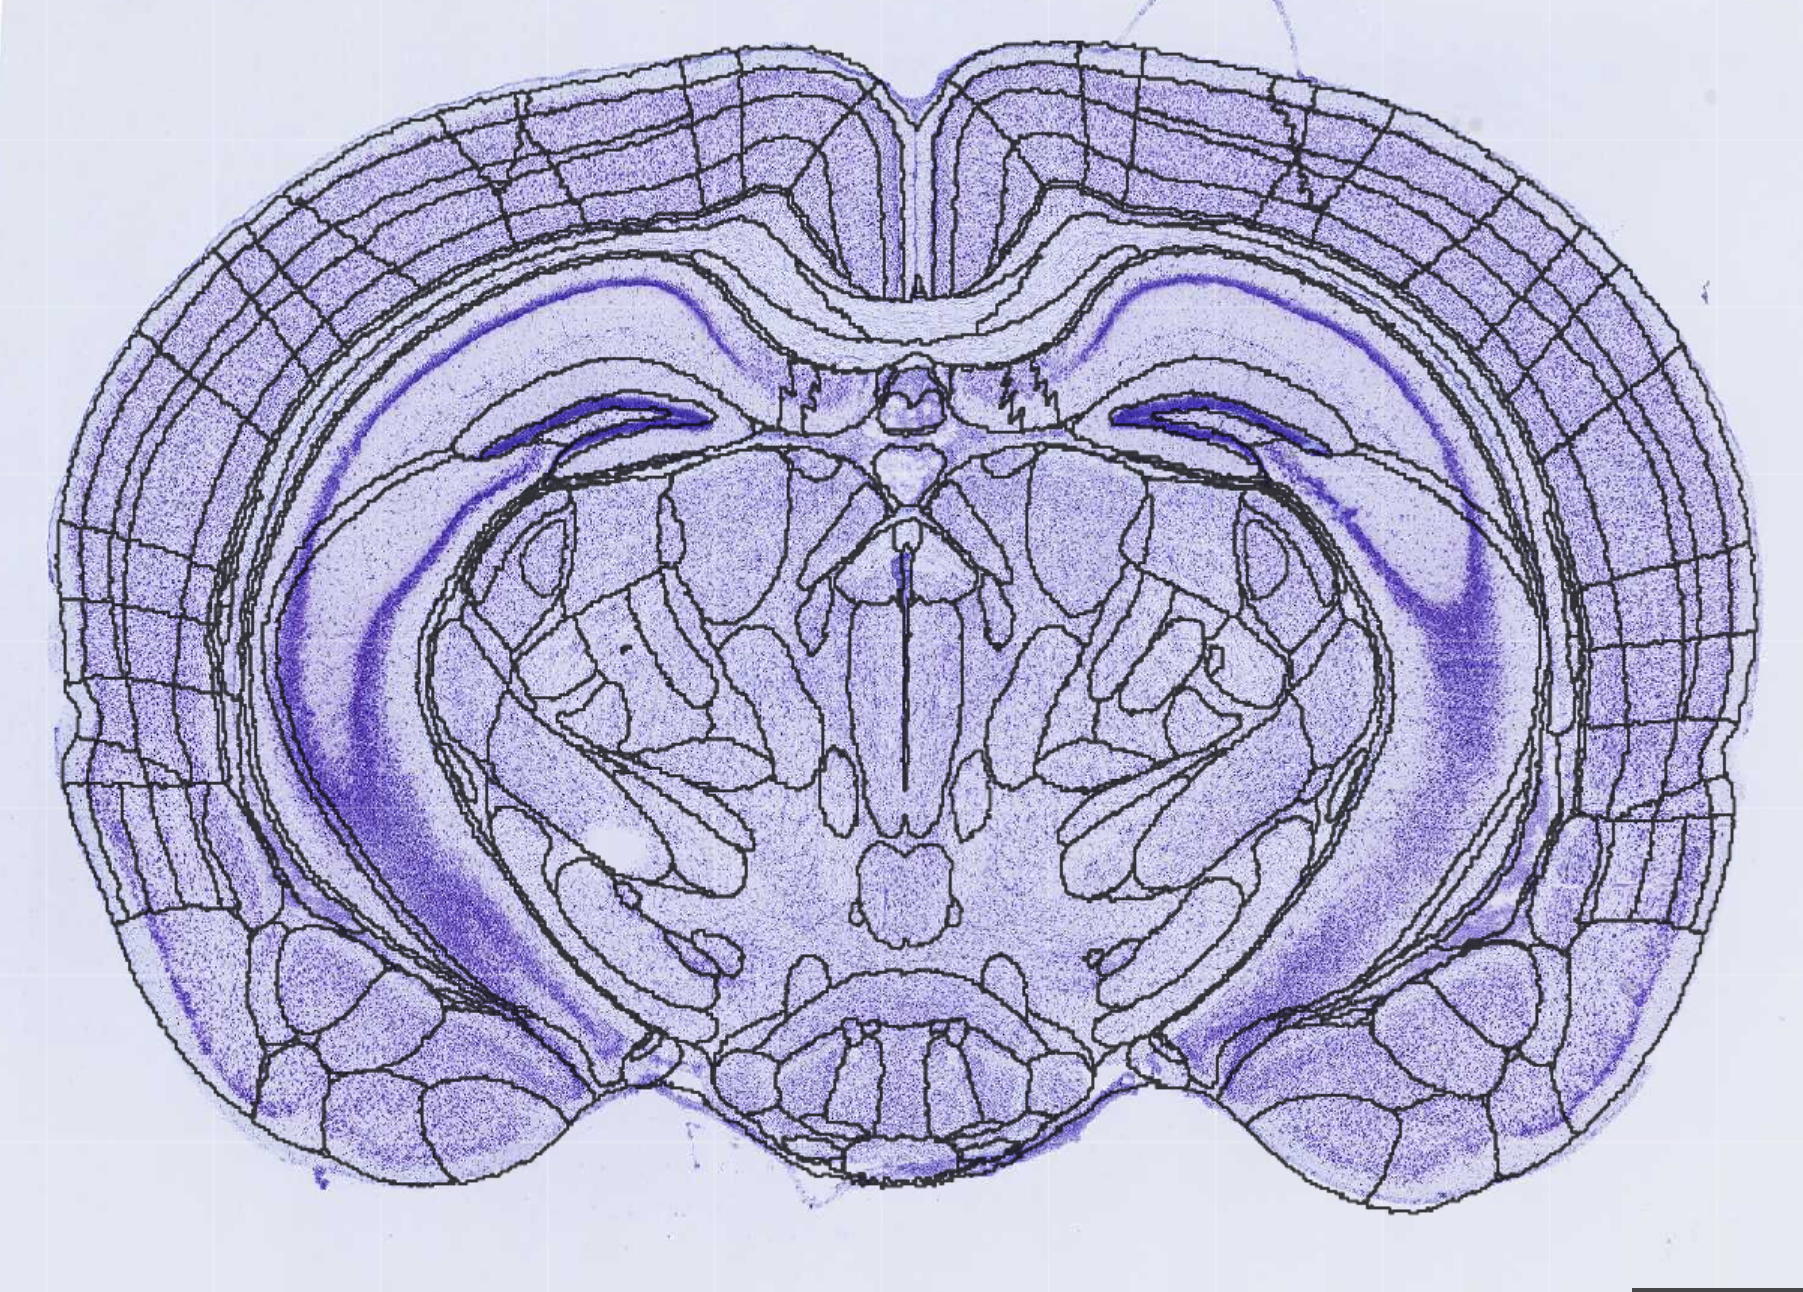
\includegraphics[width=\textwidth]{mba1.png}
\end{minipage}~
\begin{minipage}{0.7\textwidth}
ARA\\
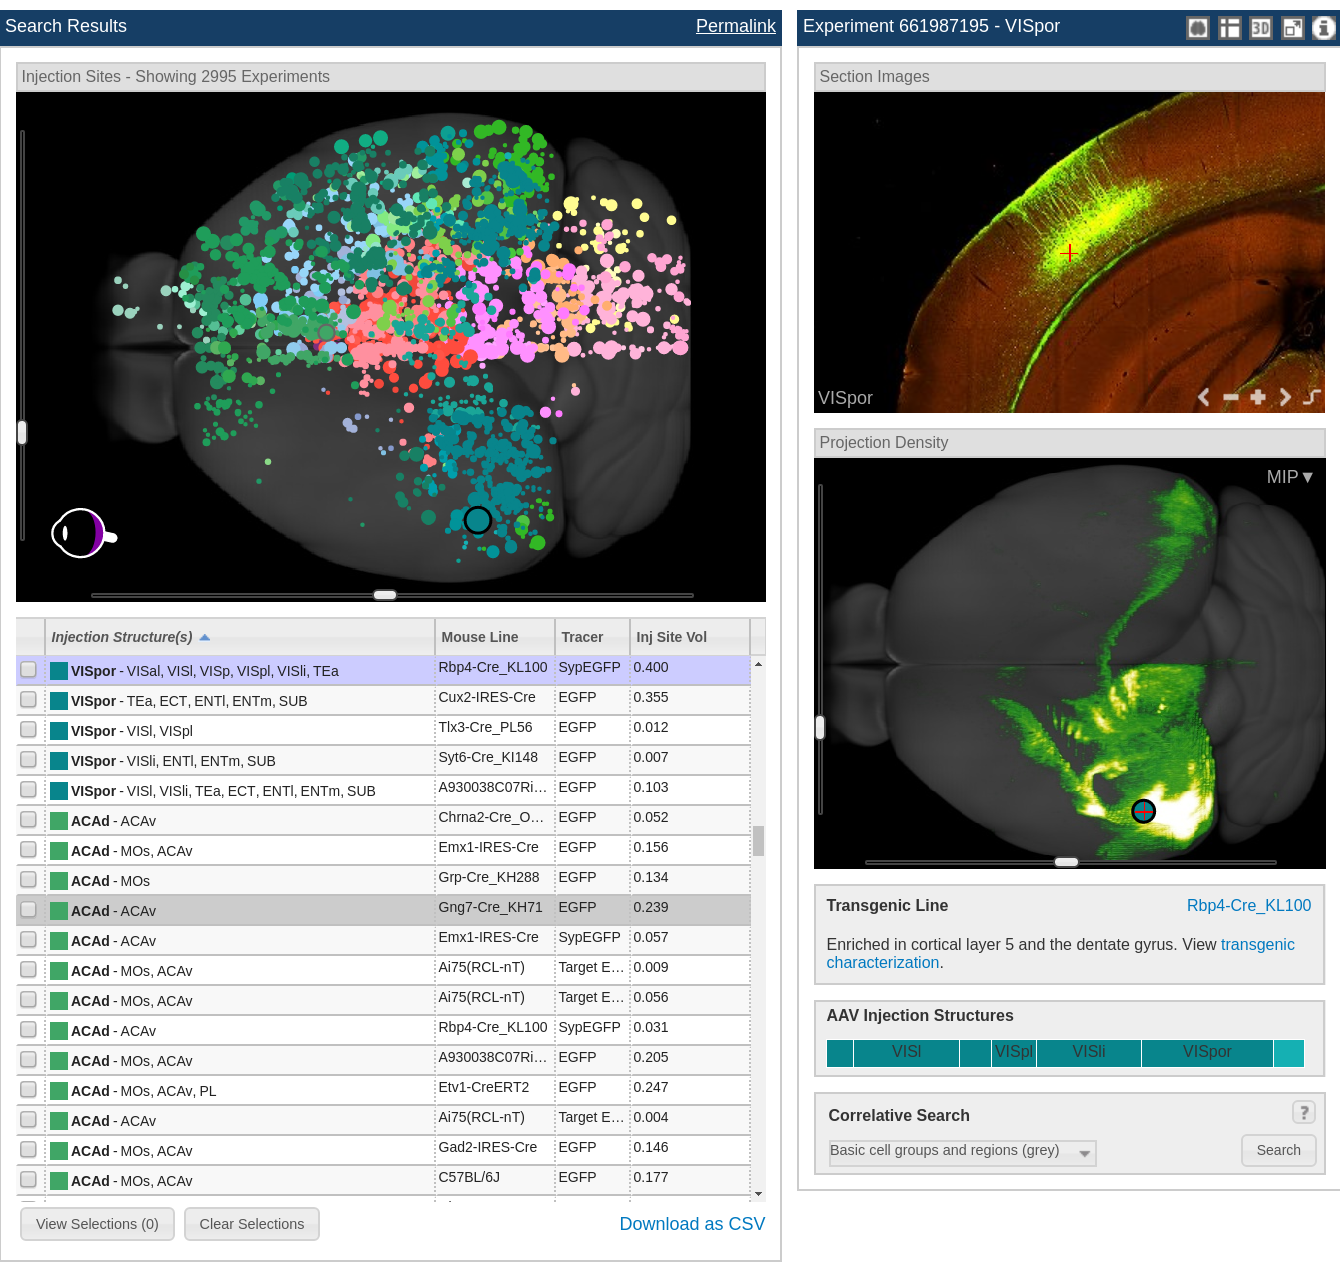
\includegraphics[width=\textwidth,clip,trim=1in 6in 1in 1.5in]{allen-connectivity}
\end{minipage}

\begin{itemize}

\item
Label images with standard ontologies

\item
Index to gene expression, cell types, tractography, etc.

\end{itemize}
\end{frame}


\begin{frame}{3. Transformation}

Studying transformations quantifies growth or atrophy %(morphometry).
\vspace{-0.5em}
\begin{center}
\only<1>{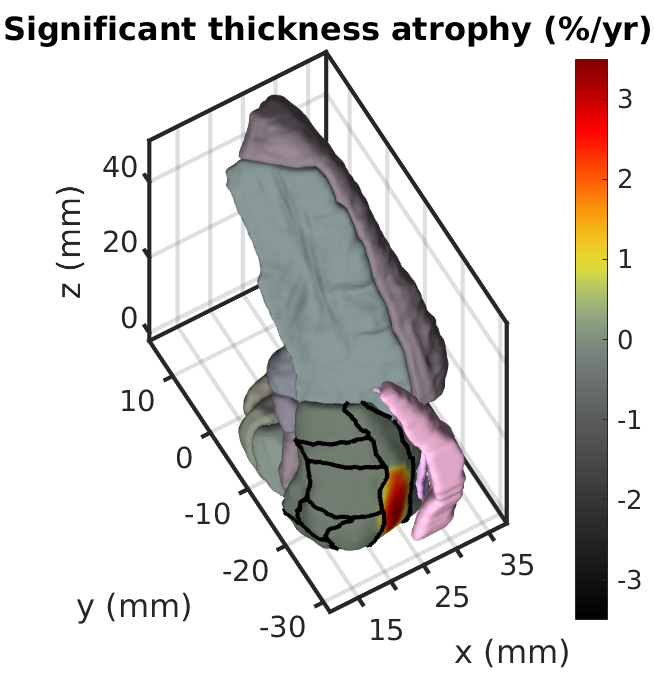
\includegraphics[width=0.45\textwidth]{v10kavli_daniel_thickness_sig.png}}%
\only<2>{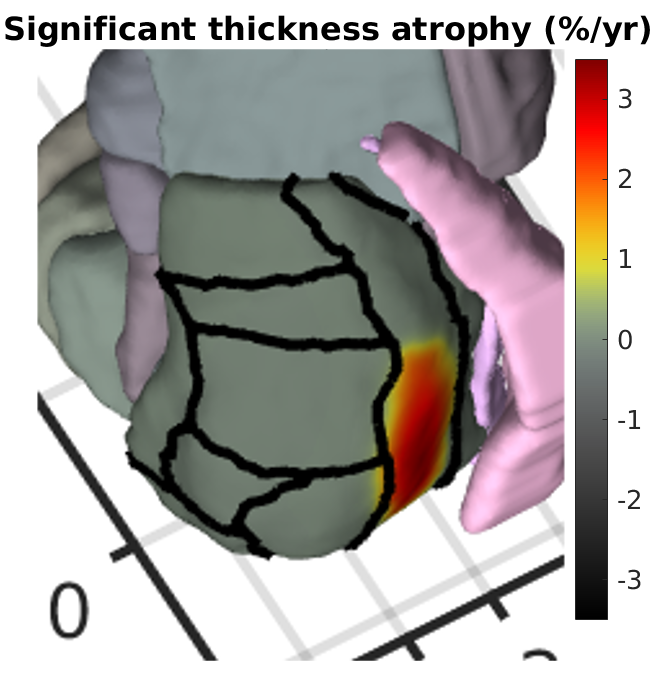
\includegraphics[width=0.45\textwidth]{v10kavli_daniel_thickness_sig-edit.png}}%
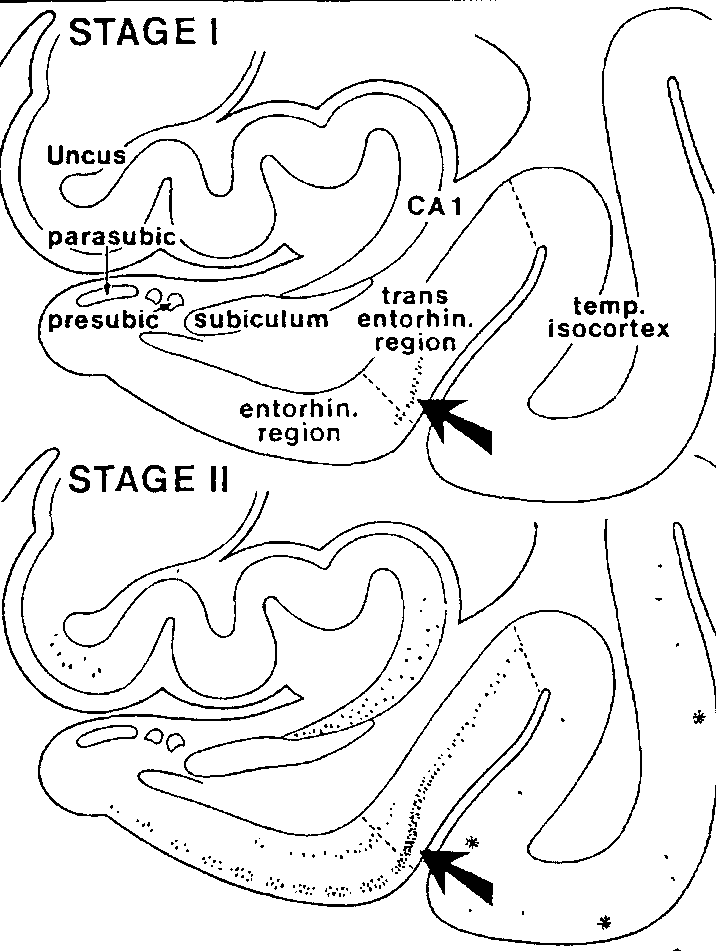
\includegraphics[width=0.3\textwidth]{braak12.png}
\end{center}
\vspace{-1em}
\begin{itemize}
\item Here thickness change in transentorhinal region measured from longitudinal MRI\footnote{Tward, Daniel J., et al. ``Entorhinal and transentorhinal atrophy in mild cognitive impairment using longitudinal diffeomorphometry.'' Alzheimer's \& Dementia: Diagnosis, Assessment \& Disease Monitoring 9 (2017): 41-50.}
\item Previously only observed at autopsy
\end{itemize}

\end{frame}










\begin{frame}{The ingredients of a brain mapping tool}

Transformation model: What types of mappings do we consider?

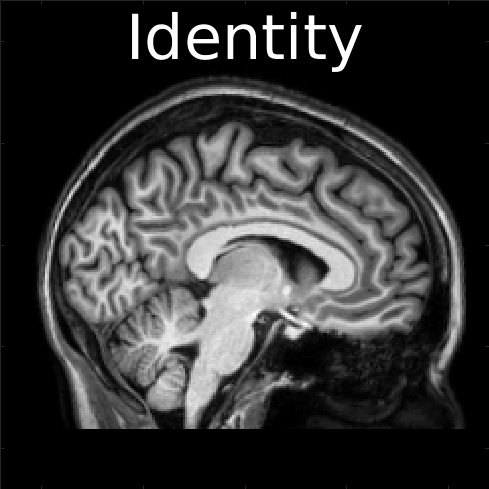
\includegraphics[width=0.15\textwidth]{ex2_id}
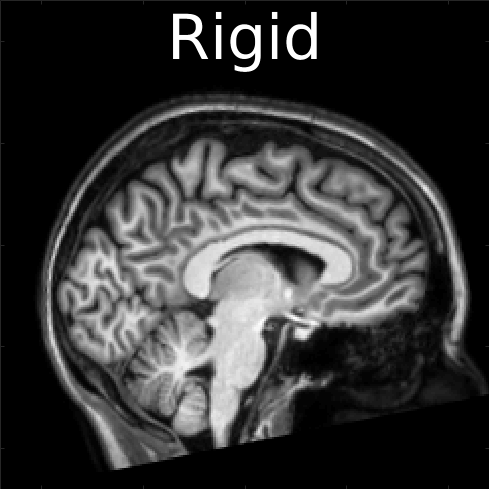
\includegraphics[width=0.15\textwidth]{ex2_rigid}
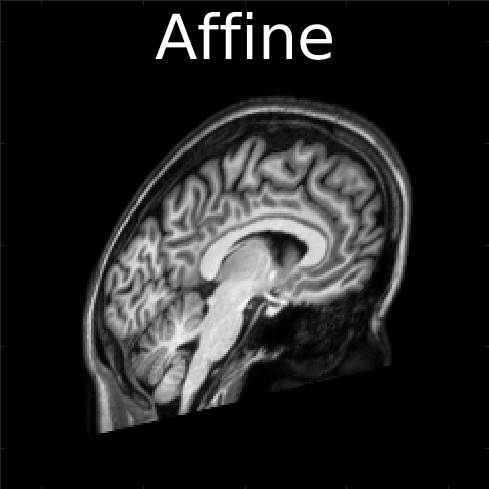
\includegraphics[width=0.15\textwidth]{ex2_affine}
%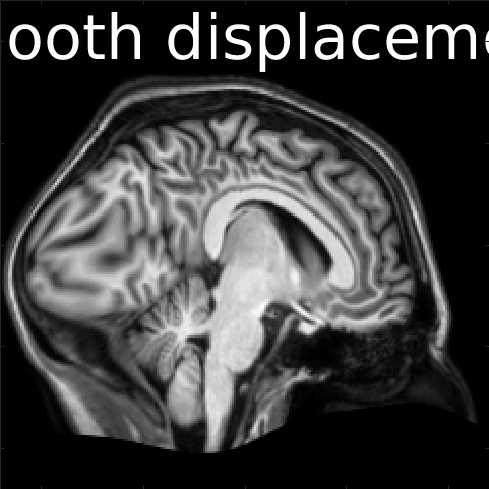
\includegraphics[width=0.2\textwidth]{ex2_disp}
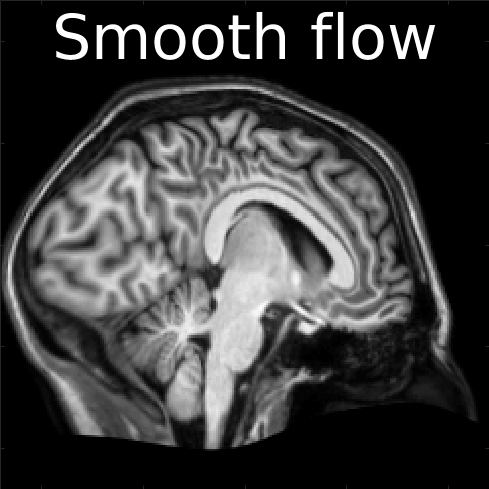
\includegraphics[width=0.15\textwidth]{ex2_flow}


\vspace{1em}
Regularization: How likely is a given transformation?

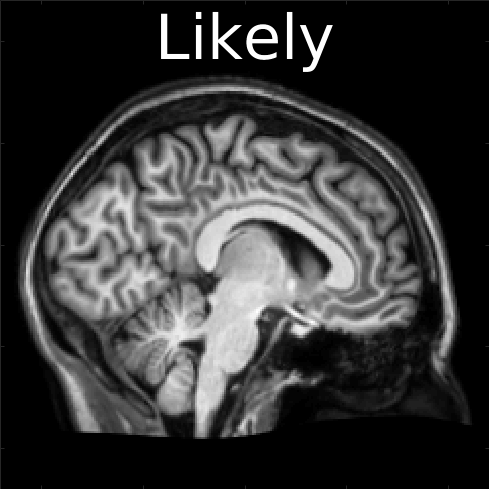
\includegraphics[width=0.15\textwidth]{ex2_flow_n_1}
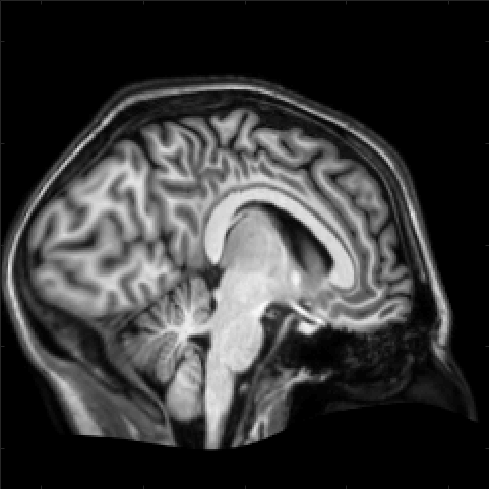
\includegraphics[width=0.15\textwidth]{ex2_flow_n_2}
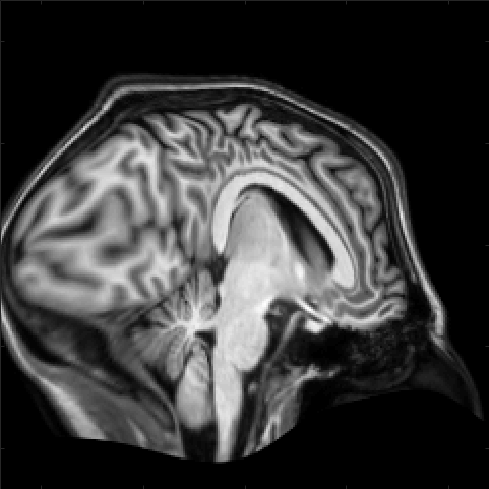
\includegraphics[width=0.15\textwidth]{ex2_flow_n_3}
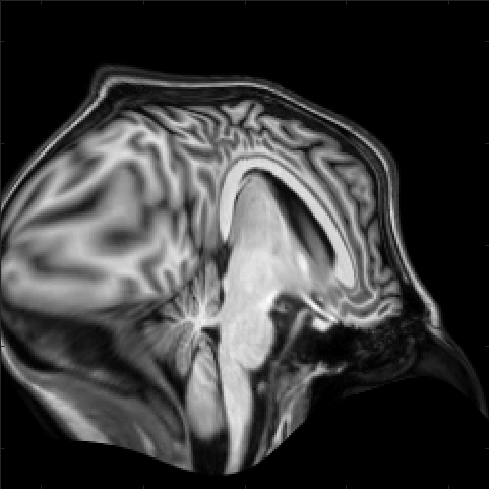
\includegraphics[width=0.15\textwidth]{ex2_flow_n_4}
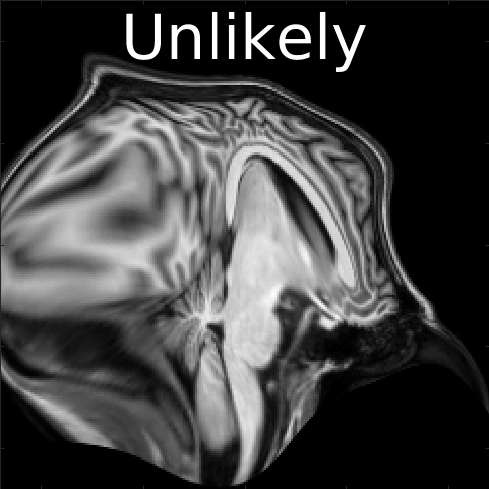
\includegraphics[width=0.15\textwidth]{ex2_flow_n_5}



\vspace{1em}
Similarity: How good is an alignment?

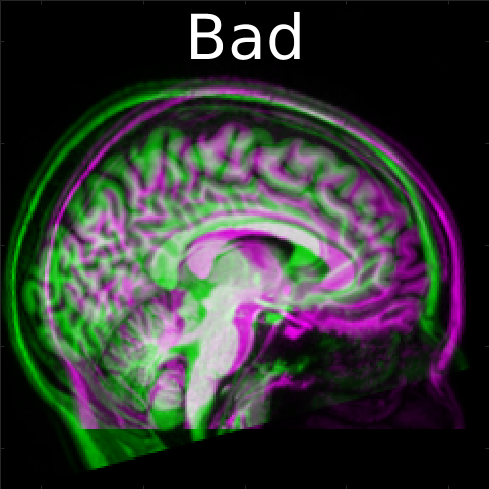
\includegraphics[width=0.15\textwidth]{ex2_affine_n_1}
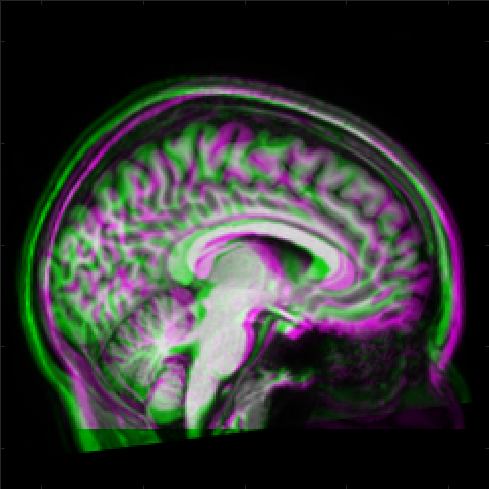
\includegraphics[width=0.15\textwidth]{ex2_affine_n_2}
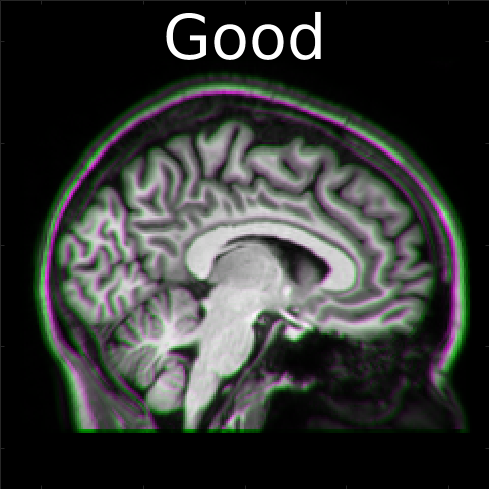
\includegraphics[width=0.15\textwidth]{ex2_affine_n_3}
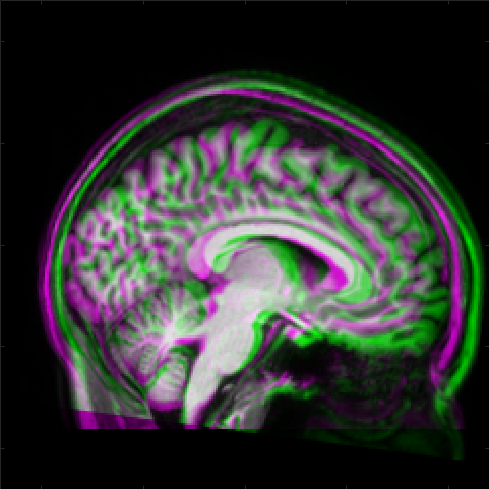
\includegraphics[width=0.15\textwidth]{ex2_affine_n_4}
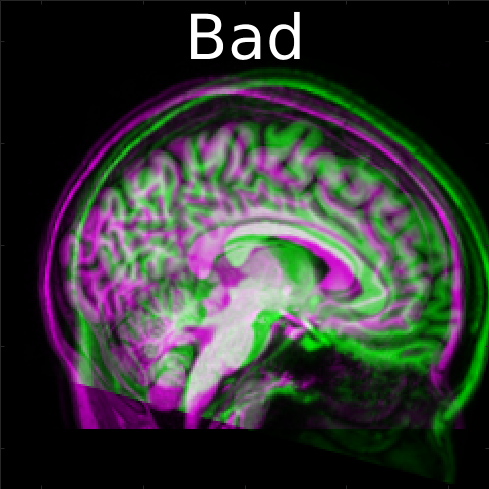
\includegraphics[width=0.15\textwidth]{ex2_affine_n_5}



\end{frame}






\begin{frame}{Challenges and solutions}

Most brain mapping techniques were developed for medical imaging, but  neuroscience data faces unique challenges:


\begin{itemize}


\item 
Incomplete or sliced data

\item 
Artifacts or damaged tissue

\item 
Multiple different modalities or appearance

\end{itemize}

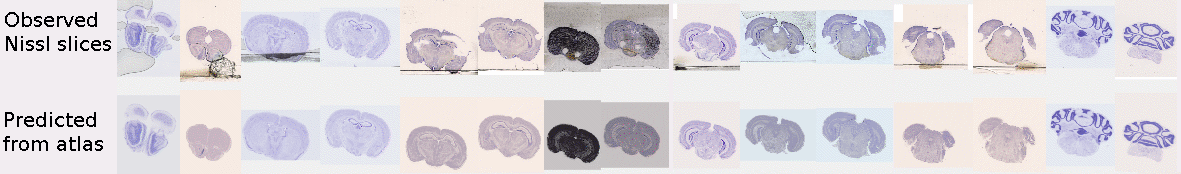
\includegraphics[width=\textwidth,clip,trim=0in 1.3in 0in 0in]{720exampleslices-edit}

\vspace{1em}

We use machine learning techniques to predict one image from another, while \alert{jointly} performing registration\footnote{ Tward, Daniel Jacob, et al. "Diffeomorphic registration with intensity transformation and missing data: Application to 3D digital pathology of Alzheimer's disease." BioRxiv (2019): 494005.}

\vspace{1em}
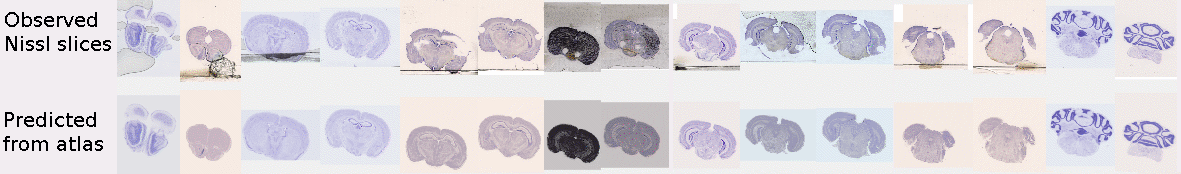
\includegraphics[width=\textwidth,clip,trim=0in 0in 0in 1.3in]{720exampleslices-edit}


\end{frame}


\begin{frame}{ARDENT\footnote{Affine and Regularized Diffeomorphic Numeric Transform.  $^5$Tward, Daniel, et al. ``Parametric surface diffeomorphometry for low dimensional embeddings of dense segmentations and imagery. IEEE transactions on pattern analysis and machine intelligence (2016) $^6$Tward, Daniel, et al. ``Estimating diffeomorphic mappings between templates and noisy data: Variance bounds on the estimated canonical volume form. Quarterly of Applied Mathematics (2019). }: NeuroData's open source brain mapping tool }

Publications and code available online from \url{neurodata.io/reg}


%\begin{itemize}
%\item Transformation model: Diffeomorphism group allows flexible deformations guaranteed smooth and invertible
%\item Similarity: Negative log likelihood allows statistical approaches to missing data and multiple modalities
%\item Regularization: Flow kinetic energy enables sparse representations effective in high dimensional bias variance tradeoff.
%\end{itemize}

\vspace{-1.5em}

\begin{table}
\begin{tabular}{p{2.1cm}p{2.3cm}p{5.3cm}}
Ingredient & Choice & Benefit\\
\hline
\hline
Transform & Diffeomorphism & Smooth invertible fluid transform\\
\hline
Similarity & Log likelihood & Enables statistical approaches to artifacts and multi-modality\\
\hline
Regularization & Kinetic energy & Enables sparse representations effective in high dimensional bias variance tradeoff$^{5,6}$
\end{tabular}
\end{table}


\vspace{-1em}

\noindent
\begin{tikzpicture}
\tikzstyle{rect} = [rectangle,text width=2.5cm,text centered];
\node (atlas) [rect] at (-4.1cm,0cm) {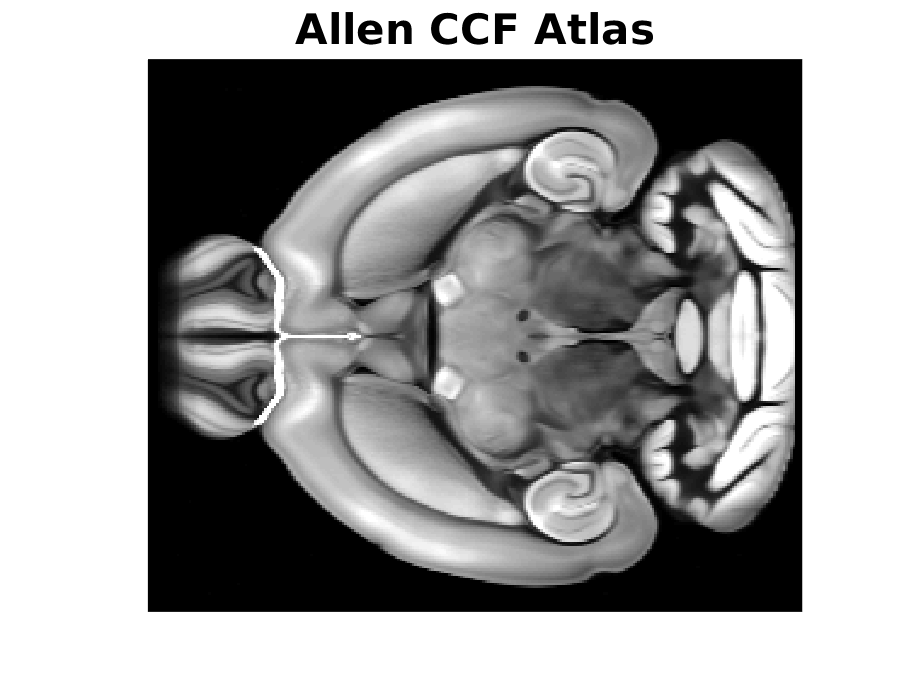
\includegraphics[width=\textwidth,clip,trim=0.5in 0in 0.5in 0in]{ardent2}};
\node (bef) [rect] at (-1.6cm,0cm) {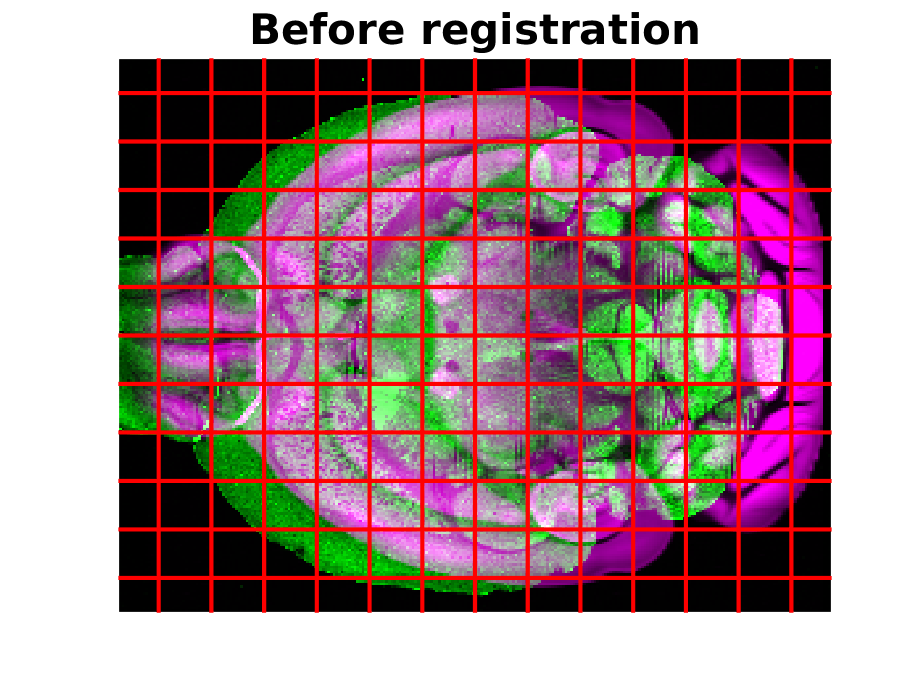
\includegraphics[width=\textwidth,clip,trim=0.5in 0in 0.5in 0in]{ardent0}};
\node (aft) [rect] at (1.6cm,0cm) {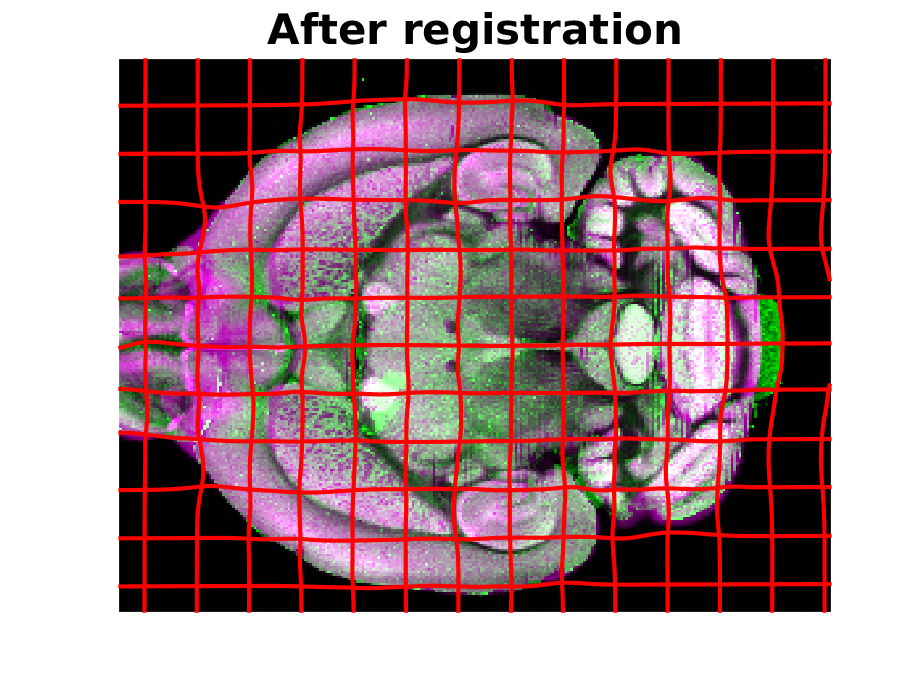
\includegraphics[width=\textwidth,clip,trim=0.5in 0in 0.5in 0in]{ardent1}};
\node (targ) [rect] at (4.1cm,0cm) {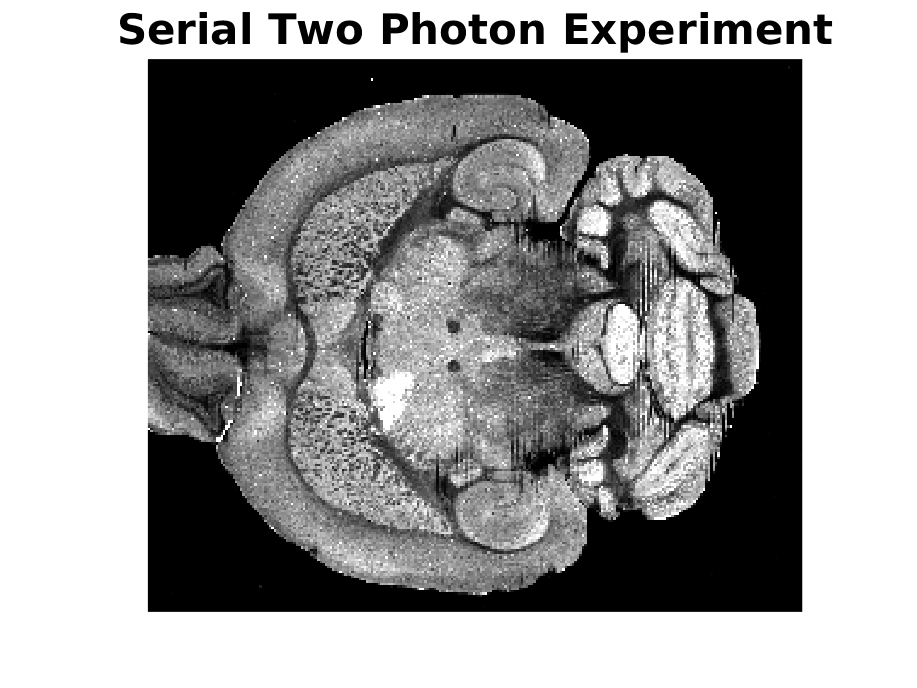
\includegraphics[width=\textwidth,clip,trim=0.5in 0in 0.5in 0in]{ardent3}};

\draw [->,thick] (bef) -- (aft);
\end{tikzpicture}

\end{frame}
\begin{frame}{Acknowledgements}

\begin{columns}
\begin{column}{0.5\textwidth}
People
\begin{itemize}
\item Michael Miller (JHU)
\item Joshua Vogelstein (JHU)
\item Susumu Mori (JHU)
\item Juan Troncoso (JHU)
\item Marilyn Albert (JHU)
\item Partha Mitra (CSHL)
\item Brian Lee (JHU)
\item Vikram Chandrashekhar (JHU)
\item Devin Crowley (JHU)

\end{itemize}
\end{column}

\begin{column}{0.5\textwidth}
Funding

\vspace{1em}

NIH: P41EB015909, R01NS086888, R01EB020062, R01NS102670, U19AG033655, R01MH105660, P50AG05146

\vspace{1em}

NSF: 16-569 NeuroNex contract 1707298, ACI1548562 (Extreme Science and Engineering Discovery Environment)

\vspace{1em}

Kavli Neuroscience Discovery Institute, BrightFocus Foundation, Dana Foundation

\end{column}
\end{columns}

\end{frame}





\end{document}